\documentclass[preprint]{aastex}
\usepackage{ctable}

\title{Sensitivity Estimates for HERA}
\author{Jonathan Pober}

\begin{document}

\section{Fiducial Array Parameters}
\label{sec:fiducial}

\ctable[caption=Fiducial System Parameters, label=params, pos=ht, mincapwidth=6in]{c|c}%
{\tnote[a]{This is the cosmological bandwidth over which the universe can
be considered co-eval, not the total instrument bandwidth.  I assume a total instrument bandwidth running from $100-200$~MHz with 1024 frequency channels.}
\tnote[b]{This is the size of a suitable cold patch in R.A. during which science observations can be conducted.}
}
{\hline
Observing Frequency & 150 MHz \\
Bandwidth & 8 MHz\tmark[a] \\
\hline
$T_{\rm receiver}$ & 100 K \\
$t_{\rm obs}$ & 120 days \\
$t_{\rm per_day}$\tmark[b] & 6 hours \\
\hline
Parabolic Element Size & 10~m \\
\hline}

Other relevant terms:
\begin{enumerate}
\item For a sky temperature model, I use $T_{\rm sky} = 569\left(\frac{\nu}{150~\rm{MHz}}\right)^{-2.5}$~K.
\item I use the following relations for a Gaussian beam model: 
\begin{equation} 
\sigma = 0.45\lambda/D
\end{equation}
\begin{equation} 
\rm{FWHM} = 2.35\sigma \\
\end{equation}
\begin{equation} 
\Omega = 1.13~\rm{FWHM} ^2
\end{equation}
\item I assume foregrounds completely contaminate all $k_{\parallel}$-modes 
below the baseline-dependent horizon limit plus an additive term of 
$0.15 h{\rm Mpc}^{-1}$.  The size of this additive term represents the
spectral ``unsmoothness'' of the sky; its value is based on the simulations
of Parsons et al. (2012).  This value may be an underestimate for the larger
elements considered here, since they will likely introduce more spectral
structure than the PAPER dipole element beams used in the simulations.
\item This sensitivity code ignores the effect of the $w$-term.  That is,
all samples which fall in the same $uv$-pixel over the course of the
observation period are treated as perfectly redundant.  Dealing with the 
complications of the $w$ term to retrieve this sensitivity is not a solved
problem.

\end{enumerate}

\section{Dense Grid of 576 Parabolic Reflectors}

The simplest array model is a dense grid of single elements.  Here we consider 
a $24\times24$ grid of parabolic reflector elements, shown in the left-hand
panel of Figure \ref{fig:p24x24}.  For comparison with the sensitivity
calculations of Parsons et al. 2012, this array has a redundancy metric
$f/f_0 = 314521.3$.  

\begin{figure}[ht]
\centering
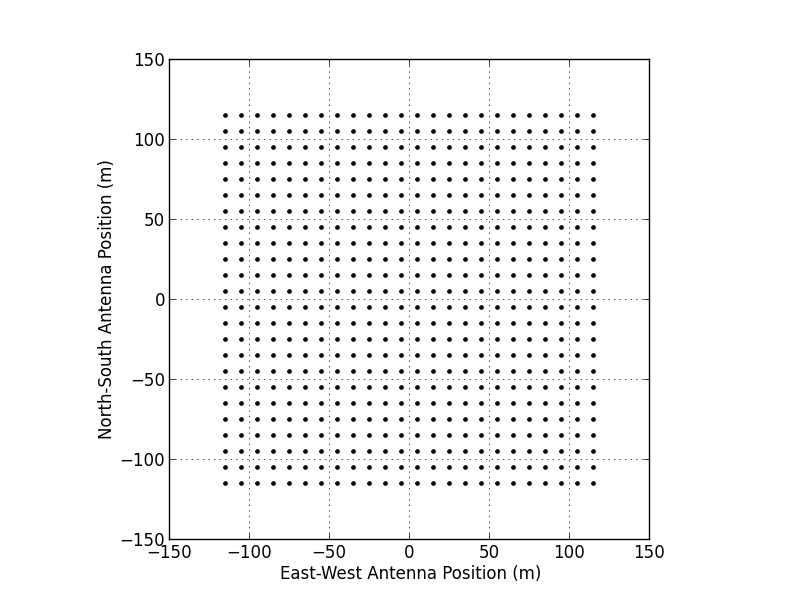
\includegraphics[width=3.5in,trim=2cm 0cm 0cm 0cm]{figures/g24x24.png}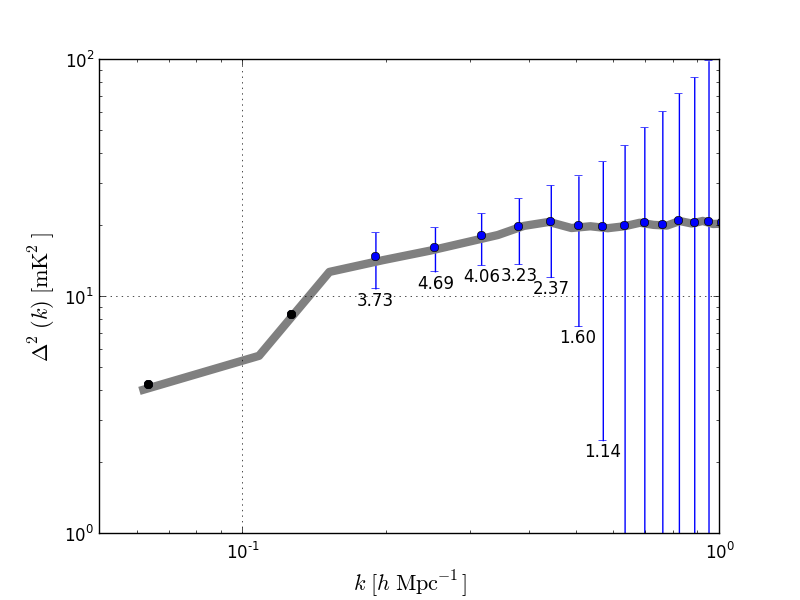
\includegraphics[width=3.5in,trim=2cm 0cm 0cm 0cm]{figures/g24x24-sense.png}
\caption{\emph{Left}: The array configuration.  \emph{Right}: The predicted 
constraints using the fiducial parameters described in \S\ref{sec:fiducial}.  
Black points are completely contaminated by foregrounds.
The numerical value below each error indicates the number of $\sigma$
significance in that particular data point.
The data are binned with a resolution of 0.063 $h\rm{Mpc}^{-1}$, corresponding
to the $k_\parallel$ resolution of the 8~MHz band.}
\label{fig:p24x24}
\end{figure}
The size of the primary 
beam of these elements is assumed to divide the six hour EoR cold patch into
6 1-hour independent fields.  The combined sensitivity of the measurement
results in an 8.6$\sigma$ detection of the EoR power spectrum.

\section{Dense Grid of 1024 Parabolic Reflectors}

Here we consider 
a $32\times32$ grid of parabolic reflector elements, shown in the left-hand
panel of Figure \ref{fig:p32x32}.  This array has a redundancy metric
$f/f_0 = 554966.5$.  
\begin{figure}[ht]
\centering
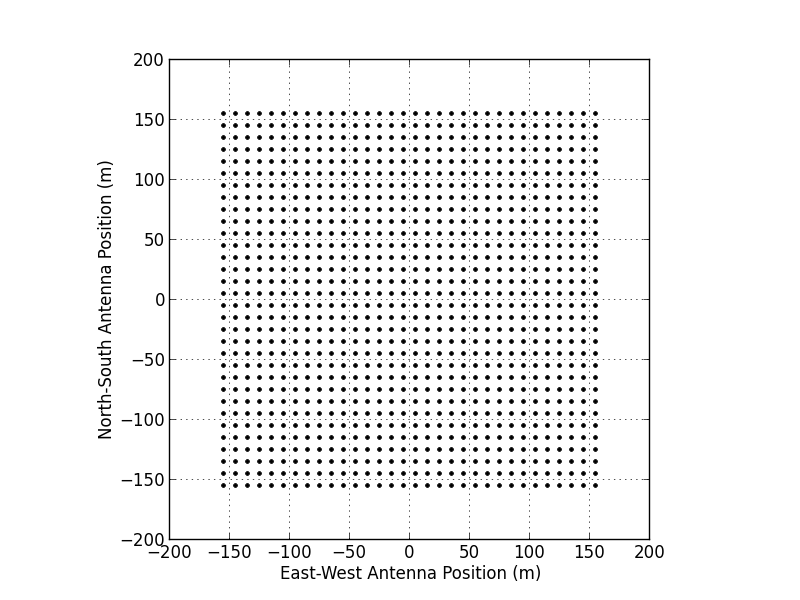
\includegraphics[width=3.5in,trim=2cm 0cm 0cm 0cm]{figures/g32x32.png}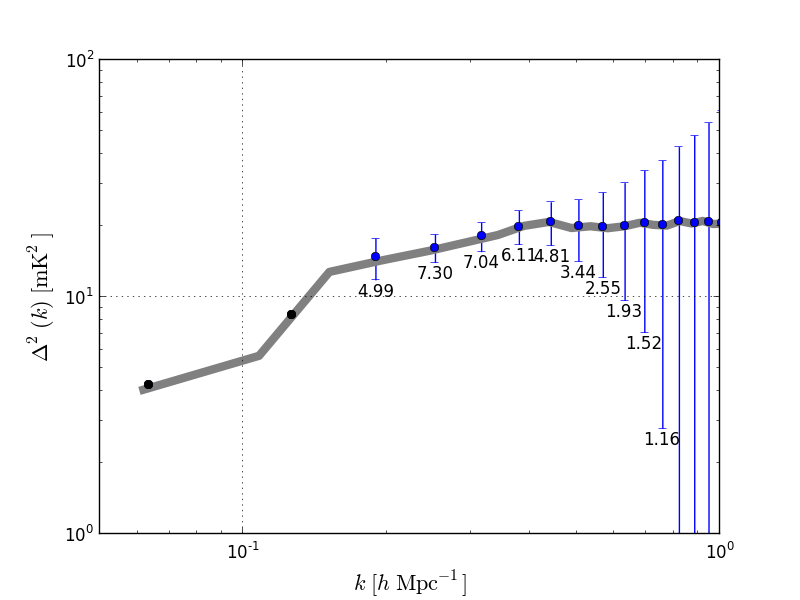
\includegraphics[width=3.5in,trim=2cm 0cm 0cm 0cm]{figures/g32x32-sense.png}
\caption{The same as Figure \ref{fig:p24x24}, but for a $32\times32$ array
of parabolic elements.}
\label{fig:p32x32}
\end{figure}
The net sensitivity results in a 14.7$\sigma$ detection of the EoR signal.

\section{Dense Grid of 512 14m Parabolic Reflectors}

The rough effect of 14m dishes is to divide the 6-hour observing window into 12
independent 30 minute fields.  Such an observation yields the following
sensitivity, with a redundancy metric of $f/f_0 = 153261.5$.  The overall
significance of the detection is 11.7$\sigma$.
\begin{figure}[ht]
\centering
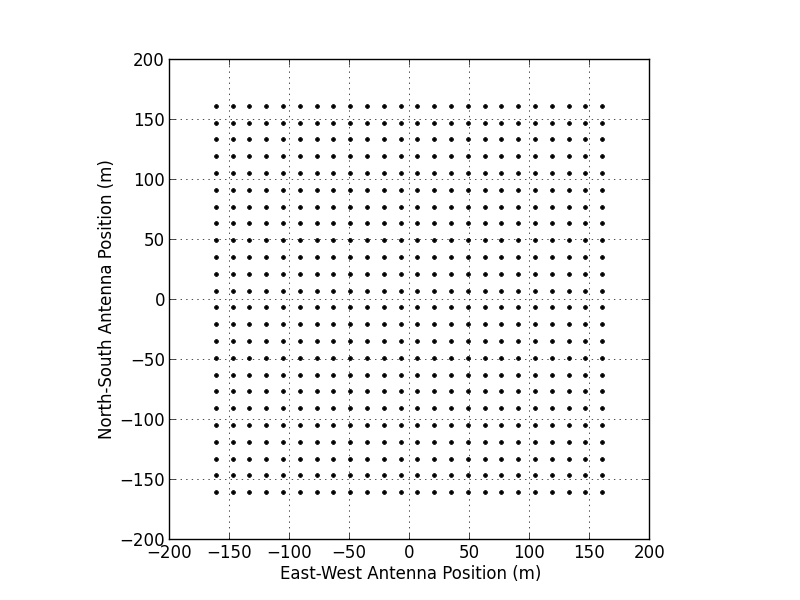
\includegraphics[width=3.5in,trim=2cm 0cm 0cm 0cm]{figures/g24x24-14m.png}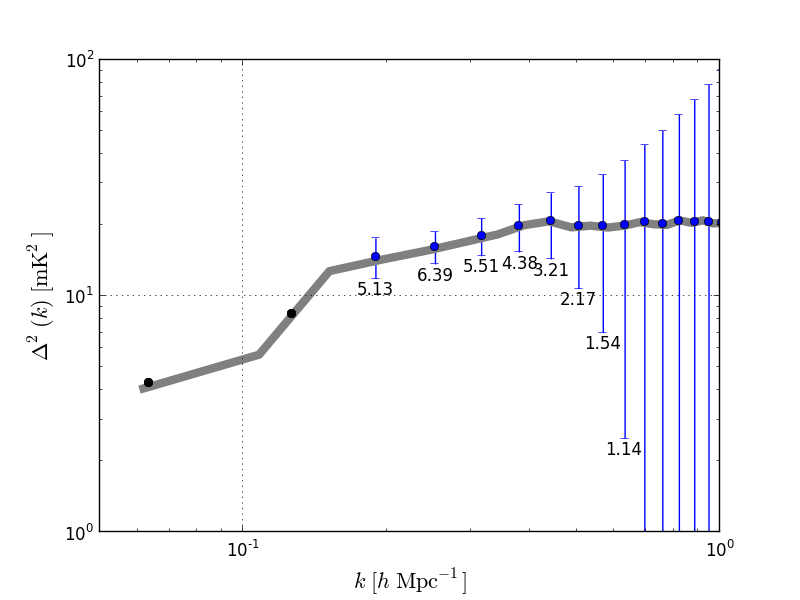
\includegraphics[width=3.5in,trim=2cm 0cm 0cm 0cm]{figures/g24x24-14m-sense.png}
\caption{The same as Figure \ref{fig:p24x24}, but for a $24\times24$ array
of 14m parabolic elements.}
\label{fig:p32x32}
\end{figure}


\end{document}
